\chapter{Evaluation}\label{evaluation}

This chapter evaluates the proposed self-explainable GNN on the 30-class
diagnosis task. Section~\ref{sec:dataset} describes the cohort and the
evaluation split. Section~\ref{sec:results} reports predictive performance
against the compared methods, analyses the per-class behaviour, and examines
explanation quality. Section~\ref{sec:eval-summary} summarises the findings.

%===============================================================
\section{Dataset Introduction}
\label{sec:dataset}
%===============================================================

The experiments use the MIMIC-IV Emergency Department
module~\cite{johnson2023mimicived}, processed into intra-patient heterogeneous
graphs as described in Chapter~\ref{implementation}. The prediction target is
the primary diagnosis, restricted to the $C = 30$ most frequent merged disease diagnosis categories. Each ED visit with a usable diagnosis label becomes one
graph.

The data is divided with the subject-aware 80/10/10 split introduced in
Section~\ref{sec:gnn-ehr}, so that all visits of a patient fall into a single
fold. The resulting sizes are summarized in Table~\ref{tab:dataset-stats}.

\begin{table}[htbp]
  \centering
  \caption{Cohort and split statistics for the 30-class disease dataset.}
  \label{tab:dataset-stats}
  \begin{tabular}{lr}
    \toprule
    Property & Value \\
    \midrule
    Number of disease classes & 30 \\
    Feature dimension $D$ & 415 \\
    Training graphs & 59{,}607 \\
    Validation graphs & 7{,}448 \\
    Test graphs & 7{,}456 \\
    Largest class (train) & 7{,}224 \\
    Smallest class (train) & 322 \\
    Class imbalance (largest : smallest) & 22.4 : 1 \\
    \bottomrule
  \end{tabular}
\end{table}

The label space is imbalanced. The largest training class holds 7{,}224 graphs
and the smallest 322, a ratio of about 22 to 1. The full per-class distribution
is reported in Appendix~\ref{app:results}. This imbalance motivates the use of
class-sensitive metrics, such as balanced accuracy and macro-F1, alongside
overall accuracy in Section~\ref{sec:results}.

%===============================================================
\section{Experimental Results and Analysis}
\label{sec:results}
%===============================================================

\subsection{Predictive Performance}
\label{sec:pred-perf}

All methods are trained and evaluated on the identical canonical split
(\texttt{comparison/\allowbreak canonical\_split.json}): the same patients, the same test
set, and the same 30 classes. Differences in the results therefore reflect the
modelling approach rather than the data. Table~\ref{tab:main-results} reports
the main comparison.

\begin{table}[htbp]
  \centering
  \small
  \setlength{\tabcolsep}{4pt}
  \caption{Predictive performance on the held-out test fold (7,456 graphs). All
    methods share the same canonical split. Best value per column among the
    completed rows in bold.}
  \label{tab:main-results}
  \begin{tabular}{lcccccc}
    \toprule
    Method & Accuracy & Balanced acc. & Macro-F1 & Micro-F1 & Top-3 & Top-5 \\
    \midrule
    Majority-class baseline & 0.1211 & 0.0333 & 0.0072 & 0.1211 & 0.3362 & 0.4606 \\
    XGBoost (tabular)       & \textbf{0.6540} & \textbf{0.6173} & \textbf{0.6066} & \textbf{0.6540} & \textbf{0.8594} & \textbf{0.9218} \\
    Plain-GCN (ablation)    & 0.5653 & 0.5754 & 0.5156 & 0.5653 & 0.7701 & 0.8456 \\
    GraphCare               & 0.5775 & 0.4454 & 0.4704 & 0.5775 & 0.7645 & 0.8403 \\
    Method~C \tbd{name}     & \tbd{} & \tbd{} & \tbd{} & \tbd{} & \tbd{} & \tbd{} \\
    ProtGNN (ours)          & 0.5632 & 0.5687 & 0.5084 & 0.5632 & 0.7696 & 0.8467 \\
    \bottomrule
  \end{tabular}
\end{table}

The six reported metrics cover both views of a 30-class imbalanced problem:
accuracy and micro-F1 measure overall correctness, balanced accuracy and
macro-F1 weight every class equally, and top-3 / top-5 accuracy measure whether
the correct diagnosis is at least ranked near the top, which is the realistic
use of a decision-support tool in an emergency department. Threshold-free
ranking metrics (AUROC, AUPRC) are not reported here because they were not
exported for all four methods; adding them would require re-running the
GraphCare and XGBoost evaluations.

Three things stand out. First, every learned method is far above the
majority-class baseline (12.1\% accuracy, 0.007 macro-F1), so the task is not
trivially solved by predicting the largest class, but the margin has to be read
against a 30-class problem where random guessing sits at 3.3\%.

Second, the two graph models trade off along different axes. GraphCare reaches
higher overall accuracy and top-$k$ ranking, while the prototype model reaches
higher balanced accuracy and macro-F1, that is, better sensitivity on the rarer
classes. Neither dominates the other.

Third, and least comfortable for the graph-based framing, the tabular XGBoost
baseline is the strongest model on all six metrics: 65.4\% accuracy against
57.8\% for the best graph model, and 0.607 macro-F1 against 0.516. Both model
families see the same clinical fields, so the gap says that the relational
structure added by the intra-patient graphs, patient-hub spokes plus PMI-linked
medication pairs, does not carry information that gradient-boosted trees cannot
already extract from the flat feature vector. What the graph models buy is not
accuracy but a decision process that can be inspected.

The ablation isolates the cost of the prototype layer. Replacing the prototype
comparison head with a standard MLP head, and keeping everything else identical
(same encoder, hyperparameters, class weighting, canonical split), gives 56.5\%
accuracy and 0.516 macro-F1 against 56.3\% and 0.508 for the prototype model.
The self-explainable head therefore costs 0.2 percentage points of accuracy and
0.008 macro-F1, which is within the run-to-run variation of this training setup
rather than a systematic loss. On this dataset the interpretability tax
discussed in Section~\ref{sec:tradeoff} is close to zero: the prototype layer
does not improve generalisation, but it does not pay for its transparency
either. \tbd{Both numbers come from a single seed. A multi-seed run
(\texttt{scripts/run\_multi\_seed.py}) would show whether the 0.2-point gap is
noise, which is what the current evidence suggests.}

\tbd{Method~C is not implemented yet; its row stays open.}

\subsection{Per-Class Behaviour and Error Analysis}
\label{sec:error-analysis}

The confusion matrix over the canonical test fold is shown in
Figure~\ref{fig:confusion}, row-normalised so each row sums to the share of that
true class. The full per-class table is in Appendix~\ref{app:results}.

Performance splits along clinical lines rather than along class frequency alone.
The classes the model handles well are the ones with a distinctive chief
complaint or medication signature: alcohol abuse with intoxication (F1 0.85),
major depressive disorder (0.83), acute pharyngitis (0.78) and GI bleed (0.73).
The classes it misses are the ones defined by a laboratory value or a systemic
state rather than by a presenting symptom: hypotension (recall 0.28), UTI or
pyelonephritis (0.34), acute kidney failure (0.36) and lower respiratory disease
(0.37). Cardiovascular risk factor, the third-largest class with 749 test
graphs, reaches only 0.41 recall, so the failure is not a small-class effect.

The most frequent confusions are within clinically adjacent groups. Back or
spine pain is predicted as limb injury or pain 58 times (6.8\% of that class),
head injury is predicted as a finger laceration 50 times (10.0\%) and as
multiple rib fractures 45 times (9.0\%), and skin or soft-tissue infection is
predicted as limb injury or pain 44 times (11.3\%). These pairs share chief
complaints (\texttt{cc[fall]}, \texttt{cc[extremity injury]},
\texttt{cc[laceration]}) and analgesic medication patterns, which is exactly the
evidence the explainers rank highest, so the errors are consistent with what the
explanations show the model using.

Class weighting has a visible cost on the precision side. Rare classes reach
usable recall but poor precision: anemia has recall 0.69 at precision 0.33,
NSTEMI 0.75 at 0.38, and acute upper respiratory infection 0.49 at 0.18. The
weighted loss pushes the model to over-predict small classes, which lifts
balanced accuracy and macro-F1, the metrics the model was selected on, while
adding false positives that a clinical deployment would notice. A cost-sensitive
threshold per class, rather than a single argmax, would be the natural next step.

\begin{figure}[htbp]
  \centering
  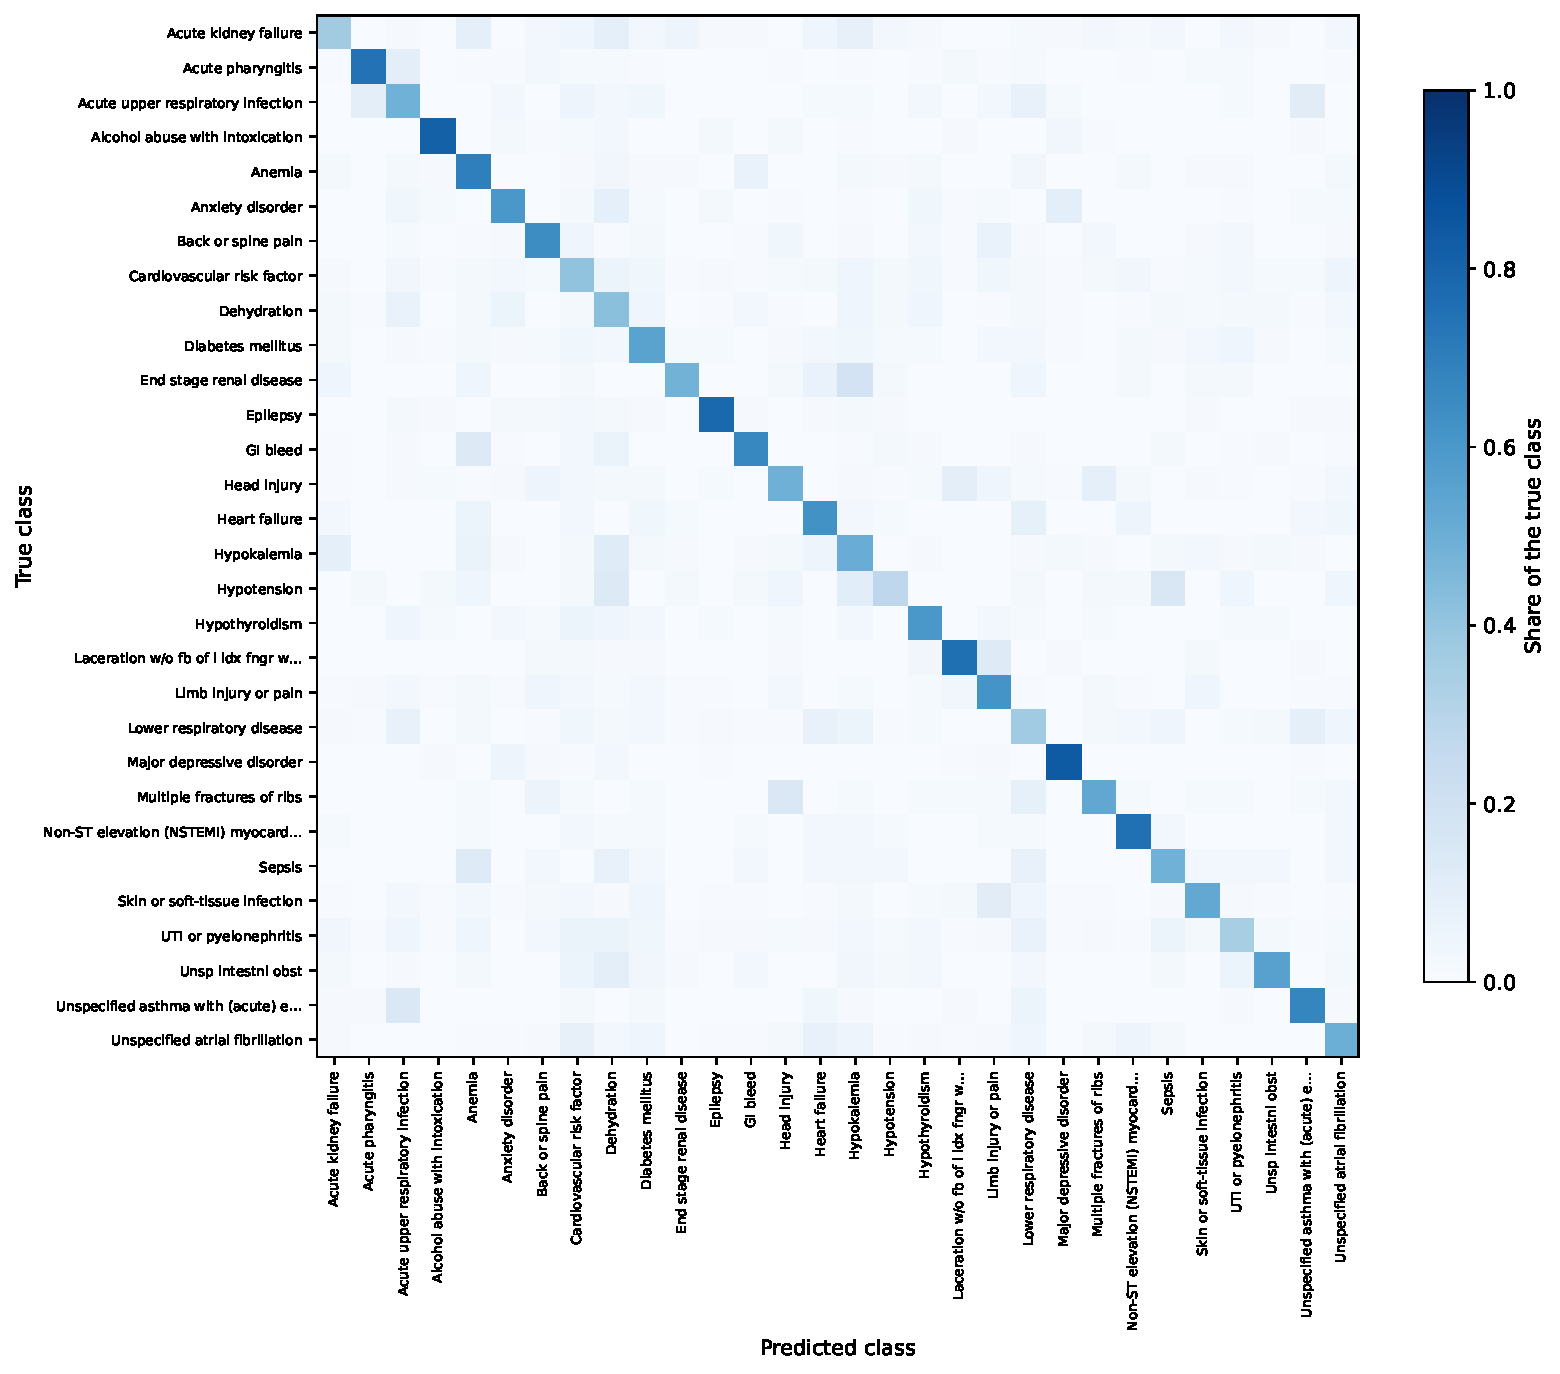
\includegraphics[width=\textwidth]{assets/confusion_matrix.pdf}
  \caption{Row-normalised confusion matrix for the prototype model on the
    canonical test fold (7,456 graphs, 30 classes). Rows are true classes,
    columns predicted classes; darker means a larger share of that true class.}
  \label{fig:confusion}
\end{figure}

\subsection{Explanation Quality}
\label{sec:expl-quality}

Because the clinical data has no ground-truth importance masks, explanation
quality is assessed through sparsity, inter-explainer agreement across the
three GraphXAI explainers, and the decoded clinical evidence
(Section~\ref{sec:eval-protocol}).

The explanation pass runs the three explainers on the first 50 graphs of the
canonical test fold, using the same checkpoint that produced the numbers in
Table~\ref{tab:main-results} (\texttt{comparison/\allowbreak
explain\_canonical.py}). Mean graph size is 21.7 nodes and 25 of the 50
predictions are correct, matching the overall test accuracy.

\caveat{\textbf{Sample size.} Unlike the predictive results, which cover the
full test fold of 7,456 graphs, every number in this section is computed on
those 50 graphs, that is 0.7\% of the test fold. The limit is GNNExplainer,
which optimises a separate mask per graph and needs several seconds per graph on
CPU, so explaining the full fold would take several hours. At $n = 50$ a
proportion such as the 32\% agreement reported below carries a 95\% confidence
interval of roughly $\pm 13$ percentage points, so the numbers below should be
read as the direction of an effect rather than as precise estimates. Every
statement in this section inherits that caveat.} \tbd{Re-run
\texttt{comparison/explain\_canonical.py --n 500} and update this section; at
$n = 500$ the same interval narrows to about $\pm 4$ points.} Sparsity is
measured as $1 - k/|V|$, where $k$ is the number of nodes carrying 90\% of the
total node-importance mass, so a higher value means the explanation concentrates
on fewer nodes. Table~\ref{tab:expl-quality} reports the results.

\begin{table}[htbp]
  \centering
  \caption{Explanation-quality summary across the three GraphXAI explainers,
    over 50 graphs of the canonical test fold \caveat{(0.7\% of it, not the full
    7,456; see the sample-size note in Section~\ref{sec:expl-quality})}. Sparsity is
    $1 - k/|V|$ at 90\% importance mass; higher means a more concentrated
    explanation. Top-node agreement is the share of graphs on which all three
    explainers rank the same node first.}
  \label{tab:expl-quality}
  \begin{tabular}{lcccc}
    \toprule
    Explainer & Mean sparsity & SD & Median & Top-node agreement \\
    \midrule
    GradExplainer            & 0.168 & 0.088 & 0.132 & \multirow{3}{*}{16/50 (32\%)} \\
    IntegratedGradExplainer  & 0.510 & 0.187 & 0.428 & \\
    GNNExplainer             & 0.563 & 0.146 & 0.550 & \\
    \bottomrule
  \end{tabular}
\end{table}

The three explainers behave differently on the same model. GNNExplainer and
Integrated Gradients concentrate the importance mass on roughly half of the
nodes, while the plain gradient explainer spreads it over almost the entire
graph: a ranking that needs 18 of 22 nodes to carry 90\% of the mass is not
something a clinician can act on.

The agreement numbers are the more informative result. All three explainers pick
the same most important node on 16 of the 50 explained graphs (32\%; \caveat{every
count in this paragraph is out of those 50, not out of the 7,456-graph test
fold}). Pairwise the rates
are similar, 52\% for the gradient explainer and GNNExplainer, 48\% for the
gradient explainer and Integrated Gradients, and 46\% for Integrated Gradients
and GNNExplainer, so no pair agrees on even two thirds of the graphs. Measured
on the top four nodes instead of the single top node, the mean overlap falls to
between 0.30 and 0.35, meaning about one of the four selected clinical factors
is shared.

This has a direct consequence for the interpretability claim. If three post-hoc
explainers applied to one fixed model disagree on which clinical entity drove
the prediction in two thirds of the cases, a single post-hoc attribution cannot
be presented as \emph{the} explanation of that prediction. The result is
consistent with the concern raised in~\cite{agarwal2023graphxai} that post-hoc
explanation quality degrades once graphs become larger and denser than the
synthetic benchmarks these methods were tuned on.

The intrinsic evidence behaves better on both counts, \caveat{on the same
50-graph sample}. The class of the nearest prototype matches the predicted class on 39 of
the 50 graphs, so the prototype layer is not decorative: it is largely what the
classifier reads. The distance
to that prototype also separates correct from incorrect predictions, averaging
0.122 when the prediction is right and 0.191 when it is wrong, which turns the
prototype evidence into a rough confidence signal that the post-hoc scores do
not provide. Because the prototypes are projected onto real training subgraphs,
that evidence is also traceable to actual patients rather than to a
reconstructed mask.

Read qualitatively, and \caveat{again over the same 50 graphs}, the decoded factors mix
clinically plausible and clinically empty signals. In a correctly predicted
finger laceration, the gradient
explainer and Integrated Gradients both rank \texttt{cc[laceration]} at the top
and the nearest three prototypes all belong to that class. Against that,
GNNExplainer ranks the patient demographic node (gender, race, transport mode)
first on most graphs, which carries no diagnostic content and mostly reflects
that the hub node aggregates the whole graph. The failure cases show the same
mechanism from the other side: a visit with an oxygen saturation almost five
standard deviations below the mean is predicted as hypokalaemia, with the
explainers pointing at a rash complaint and the patient's antiepileptic
medication instead of at the vital sign. Worked examples are given in
Appendix~\ref{app:results}.

%===============================================================
\section{Summary}
\label{sec:eval-summary}
%===============================================================

The evaluation gives three results.

On predictive performance, the tabular XGBoost baseline is the strongest model
on all six metrics (65.4\% accuracy, 0.607 macro-F1), ahead of GraphCare
(57.8\%, 0.470), the plain-GCN ablation (56.5\%, 0.516) and the prototype model
(56.3\%, 0.508). Since all four see the same clinical fields and the same test
patients, the intra-patient graph structure used here does not add predictive
information beyond what gradient-boosted trees extract from the flat feature
vector. Among the graph models the ordering depends on the metric: GraphCare
leads on overall accuracy and top-$k$ ranking, the prototype model and the
ablation on rare-class sensitivity, where both reach a balanced accuracy near
0.57 against 0.45 for GraphCare.

On the cost of interpretability, the ablation puts a number on the prototype
layer: removing it and keeping everything else fixed changes accuracy by 0.2
percentage points and macro-F1 by 0.008, in favour of the plain head. At that
size the self-explainable head is effectively free on this dataset, which is the
more useful version of the interpretability-performance trade-off than the one
usually assumed.

On explanation quality, \caveat{measured on a 50-graph sample rather than on the
full test fold}, the three post-hoc explainers disagree with each other more than they
agree: they pick the same most important node on 32\% of the explained graphs,
and their top-4 selections overlap by 0.30 to 0.35. Any single post-hoc
attribution is therefore a weak basis for a clinical claim. The intrinsic
evidence is more stable: the nearest prototype matches the predicted class on 39
of those 50 graphs and its distance separates correct from incorrect predictions
(0.122 versus 0.191), which supports the case for building the explanation into
the model rather than reconstructing it afterwards. \caveat{The gap between the
32\% explainer agreement and the 78\% prototype match is wide enough to survive
the sampling error at this size, but the individual figures are not precise
(Section~\ref{sec:expl-quality}).}

The per-class analysis adds a fourth, more clinical result: the model is
reliable on presentations with a distinctive complaint or medication signature
(alcohol intoxication, depression, pharyngitis, GI bleed, all above 0.73 F1) and
weak on states defined by laboratory values or systemic findings (hypotension,
UTI, acute kidney failure, all below 0.44 F1), which is where a decision-support
tool would need to be trusted least.

\tbd{Method~C has not been implemented, so its row in
Table~\ref{tab:main-results} and its row in Table~\ref{tab:positioning} remain
open, together with the per-class error analysis in
Section~\ref{sec:error-analysis}.}
